%
% File: chap02.tex
%
\let\textcircled=\pgftextcircled
\chapter{Results}
\label{chap:result}

\initial{T}his chapter presents the results obtained during the experiment performed on September 14th, 2016. It presents the sample's half-life, its decay constant, and the analysis from the detector, allowing us to determine the isotopic composition.

\section{Sample activity}

The data, presented in appendix~\ref{app:app01}, is plotted on figure~\ref{fig:actsample}, along with its exponential least-square fit. One can appreciate the good fit obtained, with an $R^2$ value of 99.5\%, computed using equations~\ref{eq5} to~\ref{eq8}.

\begin{figure}[t!]
	\centering
	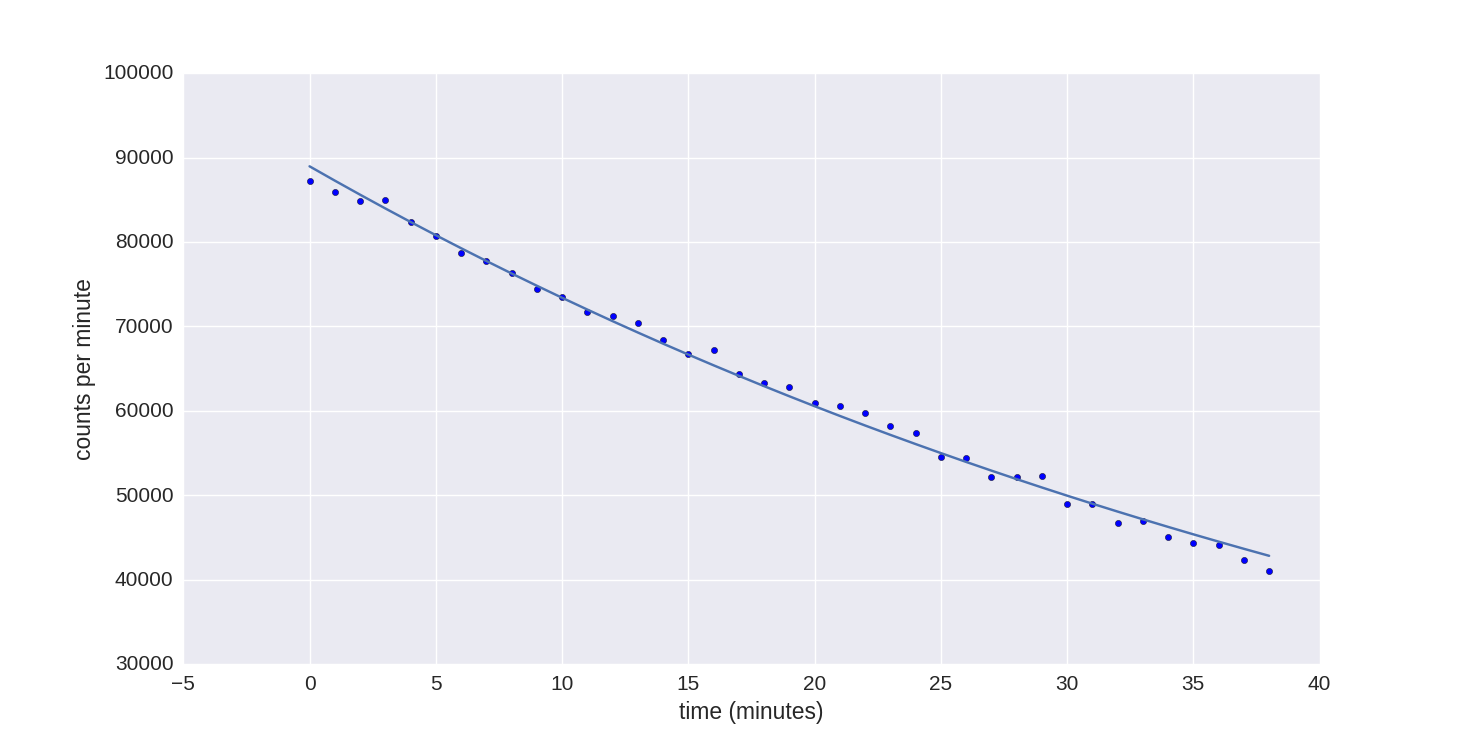
\includegraphics[height=0.4\textheight]{fig02/plot.png}
	\mycaption[Activity of the sample]{Activity of the sample.}
	\label{fig:actsample}
\end{figure}

The exponential decay of the sample follows:

\begin{equation}\label{eq9}
{A_f} = 88877.6 e^{- 0.01926 t}
\end{equation}

Using the fitted value obtained for $\lambda$, equation~\ref{eq4} gives us the sample half-life $t_{1/2}$ at 35.98 minutes. This value is of no use to us in order to determine the isotopic composition of the sample.

\section{Sample emissions}

The spectrometer use was a little less straightforward. The library is apparently missing some radioisotopes and their associated gamma ray peaks, thus it could not find the elements emitting the primary peak. Moreover, the peak analysis report is missing quite crucial information about the actual elements associated to the peaks. The results with the peaks of interests (cut off at a net peak area of 1000) are given in appendix~\ref{app:app02}.
